\chapter{Introduction}
\section{New spectrum for mobile communications}
The radio spectrum is the part of the electromagnetic spectrum used in wireless communications. These frequencies range from 20 kHz to 300 GHz and comprise technologies such as navigation, radio and television broadcasting, mobile communications, WiFi, satellite communications, etc. However, not all the spectrum frequencies have the same properties, and therefore some parts may be more valuable depending on the application.\par

Waves are affected by several phenomena, including reflection, refraction, diffraction, absorption, polarization, and scattering in different ways depending on the frequency. The most important impact that these effects have in the Ultra High Frequency (UHF) telecommunications is that as the frequency gets higher, the attenuation with distance increases, so they do not propagate so far in the environment \cite{1-01}.\par

The typically most interesting part of the spectrum for mobile telecommunications – the so-called $``$Sweetspot$"$  – is the Ultra high frequency (UHF) band which comprises from 300 MHz to 3 GHz, the decimeter band. TV broadcasting, cell phones, satellite communications, WiFi and Bluetooth are mainly allocated in UHF.

%%%%%%%%%%%%%%%%%%%% Figure/Image No: 1 starts here %%%%%%%%%%%%%%%%%%%%

\begin{figure}[H]
	\begin{Center}
		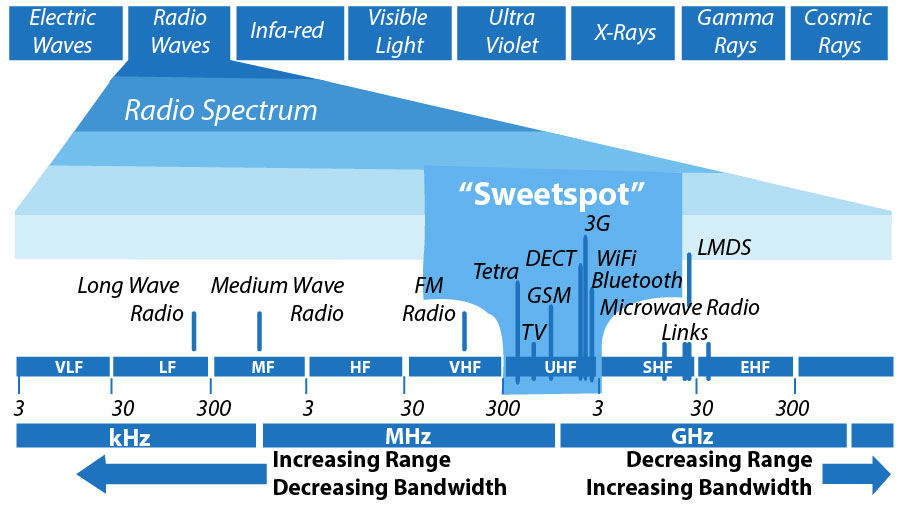
\includegraphics[width=0.95\textwidth]{./media/image1.jpeg}
		\caption{Radio spectrum's sweetspot \cite{1-34}}
	\end{Center}
\end{figure}

%%%%%%%%%%%%%%%%%%%% Figure/Image No: 1 Ends here %%%%%%%%%%%%%%%%%%%%

With the aim of reducing the interference between services, international organizations and policy-makers bind certain uses of the spectrum to small ranges of frequencies: This is called spectrum allocation. Terrestrial broadcasting used a significant part of the lower section of the UHF band in Spain, mainly 470 to 862 MHz (Considering that it also uses part of the Very High Frequency (VHF) band from 47 to 230 MHz, it is more than 50$\%$  of the spectrum below 1 GHz) \cite{1-02}. For many decades, this spectrum has been guaranteed for this terrestrial broadcasting service due to the availability of other bands for newer services and the problems to modify the existing spectrum allocation \cite{1-03}.\par

Due to the emergence of cable, satellite and Asymmetric Digital Subscriber Line (ADSL) TV, the ITU, among other international organizations, considered the need to deliver a larger number of programs with higher quality to make traditional TV broadcasting remain competitive against these newer technologies. This led to the switch from analogue TV broadcasting to digital terrestrial television \cite{1-03}.\par

Digital Terrestrial Television is based on the standard DVB-T (Digital Video Broadcasting-Terrestrial) that transmits audio, video and other information into an MPEG (Moving Picture Experts Group) transport stream. This new codification allows broadcasting to 6 digital channels with the same bandwidth that one analogue channel needed, implying more efficient spectrum management, and releasing a \textit{digital dividend} that can be used for additional TV channels and to extend the existing spectrum for mobile broadband.\par

\subsection*{The first digital dividend in Europe}
%\addcontentsline{toc}{subsection}{The first digital dividend in Europe}
In this regard, the upper part of the UHF band (790–862 MHz) was allocated to the mobile service in Region 1 in the ITU - World Radiocommunication Conference 2007 (WRC-07) \cite{1-04}. Based on this decision, the European Commission published in 2010 the Commission Decision 2010/267/UE \cite{1-05} in which \textit{\guillemotleft the 790-862 MHz band (}800 MHz band\textit{) was selected for terrestrial systems capable of providing electronic communications services in the European Union}\guillemotright .\par

Subsequently, in 2012, the European Parliament and the European Council published the decision 243/2012/EU in which forced the European members to get the digital dividend, at the latest, before 2015 \cite{1-06}.

%%%%%%%%%%%%%%%%%%%% Figure/Image No: 2 starts here %%%%%%%%%%%%%%%%%%%%

\begin{figure}[H]
	\begin{Center}
		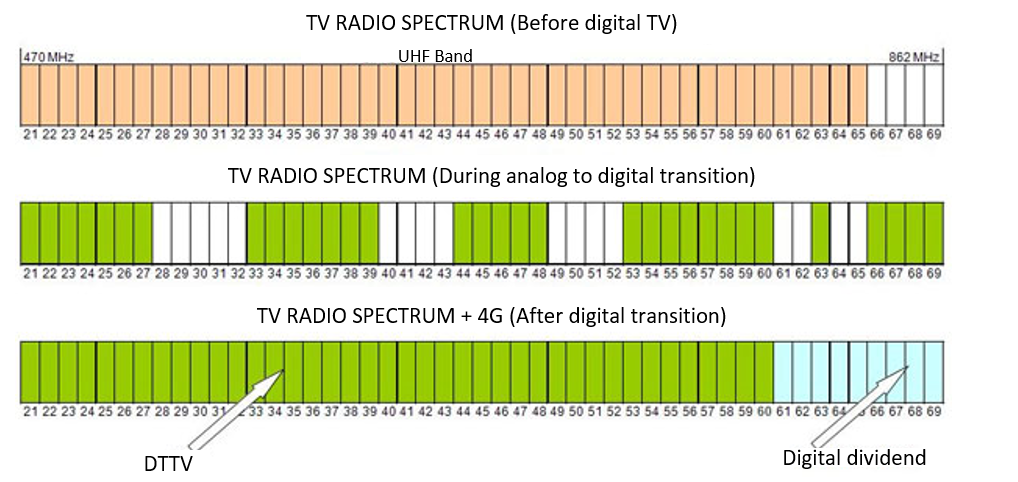
\includegraphics[width=0.95\textwidth]{./media/image2.png}
		\caption{Explanation of the Digital dividend. State Secretariat for the information society and digital agenda of Spain \cite{1-02}}
	\end{Center}
\end{figure}


%%%%%%%%%%%%%%%%%%%% Figure/Image No: 2 Ends here %%%%%%%%%%%%%%%%%%%%

Finally, the Electronic Communications Committee (ECC) within the European Conference of Postal and Telecommunications Administrations (CEPT) defined in their Report 31 \cite{1-07} their preferred harmonized frequency arrangement for the band 790-862 MHz. This arrangement would establish a downlink of 30 MHz in 6 blocks of 5 MHz each, followed by a gap of 11 MHz and an uplink of 30 MHz in 6 blocks of 5 MHz each:

%%%%%%%%%%%%%%%%%%%% Figure/Image No: 3 starts here %%%%%%%%%%%%%%%%%%%%

\begin{figure}[H]
	\begin{Center}
		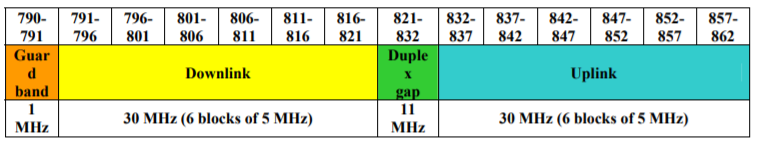
\includegraphics[width=0.95\textwidth]{./media/image3.png}
		\caption{Frequency arrangement for the 790-862 MHz band. CEPT\cite{1-07}}
	\end{Center}
\end{figure}

%%%%%%%%%%%%%%%%%%%% Figure/Image No: 3 Ends here %%%%%%%%%%%%%%%%%%%%
\subsection*{Auctions, coverage obligations, and spectrum cap}
%\addcontentsline{toc}{subsection}{Auctions, coverage obligations, and spectrum cap}
The European Member States started to develop national strategies to allocate the new spectrum (790–862 MHz) to the MNOs (Mobile Network Operators) in their countries. The terms and conditions fixed by the European Union were intended to \guillemotleft \textit{foster the collective use of spectrum as well as shared use of spectrum}\guillemotright , \guillemotleft \textit{enhance flexibility}\guillemotright  and \guillemotleft \textit{promote competition, investment and the efficient use of spectrum as a public good}\guillemotright  \cite{1-06}.\par

In this case, most governments decided to allocate spectrum through an auction procedure. The advantages of auctions are the promotion of competition and the more transparent of the spectrum since there is no subjectivity in the process. It also provides an important amount of money to governments since the competition among several bidders generally leads to higher bids. The ITU presentation in \cite{1-08} shows examples of auctions of the 800 MHz band in Europe:

%%%%%%%%%%%%%%%%%%%% Table No: 2 starts here %%%%%%%%%%%%%%%%%%%%

{
\setlength\extrarowheight{3pt}
\begin{longtable}{p{1.42in}p{1.8in}p{1.36in}}
\caption{Results of the spectrum auctions of the 800MHz band in Europe. ITU \cite{1-08}}
\endfirsthead
\multicolumn{3}{c}{\textit{continued from previous page}}\hline
\endhead\hline
\multicolumn{3}{r}{\textit{continued on next page}} \\
\endfoot
\hline 
\endlastfoot\hline
%row no:1
\multicolumn{1}{|p{1.42in}}{\Centering \textbf{Country}} & 
\multicolumn{1}{|p{1.8in}}{\Centering \textbf{Amount of auction in €}} & 
\multicolumn{1}{|p{1.36in}|}{\Centering \textbf{Year of auction}} \\
\hhline{---}
%row no:2
\multicolumn{1}{|p{1.42in}}{\Centering Austria} & 
\multicolumn{1}{|p{1.8in}}{\Centering 2,000 M€} & 
\multicolumn{1}{|p{1.36in}|}{\Centering October 2013} \\
\hhline{---}
%row no:3
\multicolumn{1}{|p{1.42in}}{\Centering Belgium} & 
\multicolumn{1}{|p{1.8in}}{\Centering 360 M€} & 
\multicolumn{1}{|p{1.36in}|}{\Centering November 2013} \\
\hhline{---}
%row no:4
\multicolumn{1}{|p{1.42in}}{\Centering Croatia} & 
\multicolumn{1}{|p{1.8in}}{\Centering 40 M€} & 
\multicolumn{1}{|p{1.36in}|}{\Centering September 2012} \\
\hhline{---}
%row no:5
\multicolumn{1}{|p{1.42in}}{\Centering Czech Republic} & 
\multicolumn{1}{|p{1.8in}}{\Centering 266 M€} & 
\multicolumn{1}{|p{1.36in}|}{\Centering November 2013} \\
\hhline{---}
%row no:6
\multicolumn{1}{|p{1.42in}}{\Centering Denmark} & 
\multicolumn{1}{|p{1.8in}}{\Centering 99 M€} & 
\multicolumn{1}{|p{1.36in}|}{\Centering 2012} \\
\hhline{---}
%row no:7
\multicolumn{1}{|p{1.42in}}{\Centering Finland} & 
\multicolumn{1}{|p{1.8in}}{\Centering 108 M€} & 
\multicolumn{1}{|p{1.36in}|}{\Centering October 2013} \\
\hhline{---}
%row no:8
\multicolumn{1}{|p{1.42in}}{\Centering France} & 
\multicolumn{1}{|p{1.8in}}{\Centering 2,600 M€} & 
\multicolumn{1}{|p{1.36in}|}{\Centering December 2011} \\
\hhline{---}
%row no:9
\multicolumn{1}{|p{1.42in}}{\Centering Germany} & 
\multicolumn{1}{|p{1.8in}}{\Centering 3,570 M€} & 
\multicolumn{1}{|p{1.36in}|}{\Centering 2010} \\
\hhline{---}
%row no:10
\multicolumn{1}{|p{1.42in}}{\Centering Ireland} & 
\multicolumn{1}{|p{1.8in}}{\Centering 854 M€} & 
\multicolumn{1}{|p{1.36in}|}{\Centering 2012} \\
\hhline{---}
%row no:11
\multicolumn{1}{|p{1.42in}}{\Centering Italy} & 
\multicolumn{1}{|p{1.8in}}{\Centering 2,960 M€} & 
\multicolumn{1}{|p{1.36in}|}{\Centering January 2013} \\
\hhline{---}
%row no:12
\multicolumn{1}{|p{1.42in}}{\Centering Lithuania} & 
\multicolumn{1}{|p{1.8in}}{\Centering 2,4 M€} & 
\multicolumn{1}{|p{1.36in}|}{\Centering October 2013} \\
\hhline{---}
%row no:13
\multicolumn{1}{|p{1.42in}}{\Centering Netherlands} & 
\multicolumn{1}{|p{1.8in}}{\Centering 3,800 M€} & 
\multicolumn{1}{|p{1.36in}|}{\Centering December 2012} \\
\hhline{---}
%row no:14
\multicolumn{1}{|p{1.42in}}{\Centering Portugal} & 
\multicolumn{1}{|p{1.8in}}{\Centering 270 M€} & 
\multicolumn{1}{|p{1.36in}|}{\Centering 2012} \\
\hhline{---}
%row no:15
\multicolumn{1}{|p{1.42in}}{\Centering Romania} & 
\multicolumn{1}{|p{1.8in}}{\Centering 682 M€} & 
\multicolumn{1}{|p{1.36in}|}{\Centering September 2012} \\
\hhline{---}
%row no:16
\multicolumn{1}{|p{1.42in}}{\Centering Spain} & 
\multicolumn{1}{|p{1.8in}}{\Centering 1,300 M€} & 
\multicolumn{1}{|p{1.36in}|}{\Centering July 2015} \\
\hhline{---}
%row no:17
\multicolumn{1}{|p{1.42in}}{\Centering Sweden} & 
\multicolumn{1}{|p{1.8in}}{\Centering 233 M€} & 
\multicolumn{1}{|p{1.36in}|}{\Centering 2009} \\
\hhline{---}
%row no:18
\multicolumn{1}{|p{1.42in}}{\Centering Switzerland} & 
\multicolumn{1}{|p{1.8in}}{\Centering CHF 996 Million} & 
\multicolumn{1}{|p{1.36in}|}{\Centering July 2005} \\
\hhline{---}
%row no:19
\multicolumn{1}{|p{1.42in}}{\Centering The UK} & 
\multicolumn{1}{|p{1.8in}}{\Centering 2,700 M€} & 
\multicolumn{1}{|p{1.36in}|}{\Centering February 2013} \\
\hhline{---}


\end{longtable}}
%%%%%%%%%%%%%%%%%%%% Table No: 2 ends here %%%%%%%%%%%%%%%%%%%%

For a deeper study of the benefits of the different kinds of auctions, the reader is referred to \cite{1-09}.\par

Due to the favourable propagation properties of the 800 MHz band, the European Union Multiannual Radio Spectrum Policy [1-06] article 3c) state that the Member States should \guillemotleft \textit{foster access to broadband at a speed of not less than 30 Mbps by 2020 for all Union citizens}\guillemotright \textit{. }This decision is focused on homogenizing the end-user speed of the mobile network, so that the difference between the urban areas, with higher speeds, and rural areas, with lower speeds, can be reduced. \par

Even though each country implemented different variations of this policy, most of the biggest countries in Europe imposed some coverage and rollout obligations for those MNOs that sought access to blocks at 800 MHz. For example, the Spanish government obliged MNOs to elaborate a report on how they will jointly meet this requirement \cite{1-10} and the office of communications of UK (Ofcom) set a 95$\%$  population coverage with at least 2 Mbps in each of the UK nations in one of the blocks \cite{1-11}. These coverage obligations will be examined in greater detail in the following chapters.\par

Spectrum integration is the last characteristic of the spectrum auction in Europe. Most governments imposed a certain cap to ensure that this natural resource is distributed among the principal MNOs. In most countries, it was set as a limit on the amount of spectrum that each operator could hoard across all the bands, as a cap in a specific band or as a combination of both. In the following chapters, this spectrum cap will be examined for all the countries under study. This paper of the Global System for Mobile Communications (GSMA) \cite{1-11} covers the historical evolution of the spectrum cap worldwide.\par

\section{5G}
%\addcontentsline{toc}{subsection}{5G}
Initially, mobile networks were mainly intended for voice. As technology evolved, users began to use mobile phones for more purposes: web browsing was standardized in 3G, and 4G allowed users to consume higher-speed data and video streaming, among other examples. This increasing trend is expected to be even more pronounced now, given the emergence of technologies such as 4K video streaming and virtual and augmented reality, that will require higher bandwidth and capacity \cite{1-14}. Moreover, according to the VNI (Visual Networking Index) of Cisco \cite{1-15}, mobile data traffic will increase sevenfold between 2016 and 2021 and Video-on-Demand (VoD) traffic will nearly double by 2021.\par

Apart from the natural growth of the data traffic demand, the industry is aiming to develop new communication technologies with extremely low latency, ultra-reliable communications with low latencies or that could allow for a higher density of devices connected to the network. These features will enable the development of new possibilities such as smart cities, cooperative automated driving, and, as well as to enable the full potential of the Internet of Things \cite{1-16}.\par

Therefore, the following three main potential use cases \cite{1-17} upon technical requirements have been defined:\par

\begin{itemize}
	\item Use case 1: Enhanced mobile broadband\par

This scenario focuses on providing very high data rates for future mobile broadband users to experience instantaneous connectivity without delays. Data rates considered are at least 1 Gb/s or more to support ultrahigh-definition video, virtual reality applications and even more speed to support mobile cloud services. \par

	\item Use case 2: Massive machine-type communications\par

This scenario focuses on the efficient handling of a very large number of devices (including, e.g., machine type devices and sensors) with widely varying requirements. Current mobile network systems capacity should expand to support several billions of applications and hundreds of billions of machines connected simultaneously. \cite{1-18} This will enable a faster development of Smart Cities, Smart Logistics, and Intelligent Agriculture.\par

	\item Use case 3: Ultra-reliable and low latency communications\par

This scenario focuses on new applications and use cases with very strict requirements on latency and reliability. Networks with less than one-millisecond latency would enable to support real-time mobile control, vehicle-to-vehicle applications and communications and robotic-assisted surgery among others.\par

5th generation mobile networks are the proposed next communication standards that will allow all these industry developments to take place. This triangle is commonly used to show all the scenarios in which the 5G is intended to be the real technology standard of the near future:

%%%%%%%%%%%%%%%%%%%% Figure/Image No: 4 starts here %%%%%%%%%%%%%%%%%%%%

\begin{figure}[H]
	\begin{Center}
		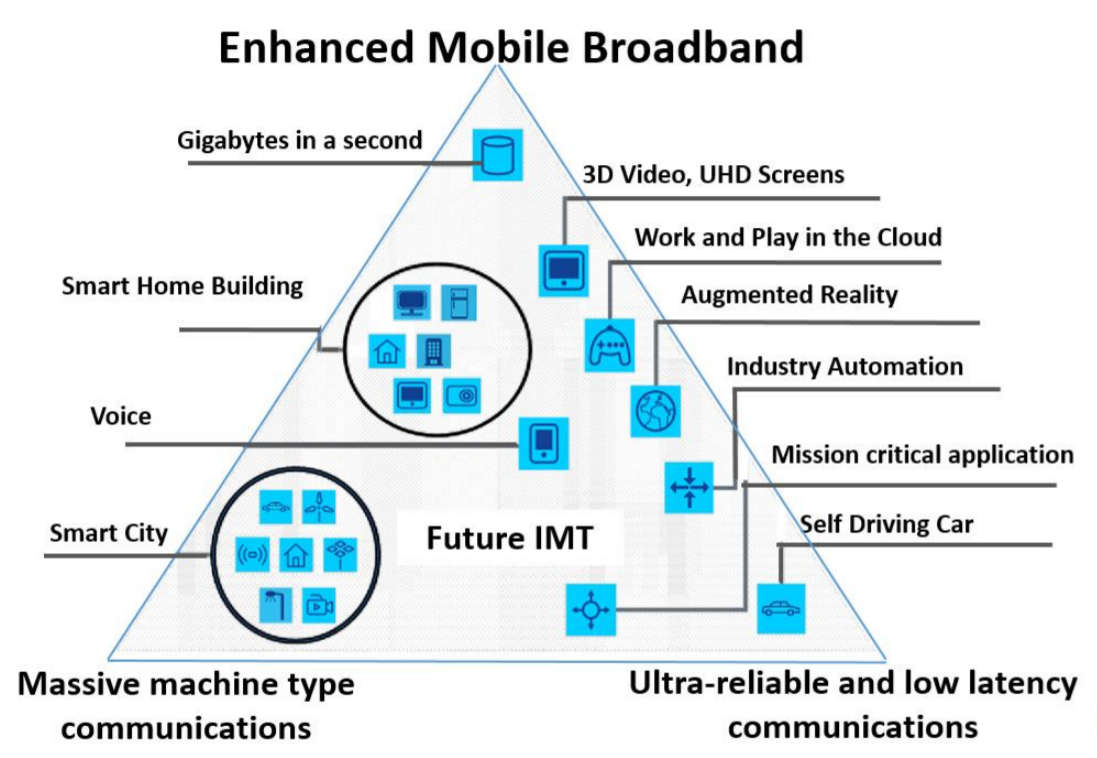
\includegraphics[width=0.95\textwidth]{./media/image4.png}
		\caption{Potential use cases of the 5G networks. ITU-T workshops April 2017\cite{1-17}}
	\end{Center}
\end{figure}


%%%%%%%%%%%%%%%%%%%% Figure/Image No: 4 Ends here %%%%%%%%%%%%%%%%%%%%

\end{itemize}
\section{Radio Spectrum for 5G}
%\addcontentsline{toc}{subsection}{Radio Spectrum for 5G}
Although the mobile industry, academic institutions, and international standard-making bodies are developing technologies that will be central to 5G, the success of the service rollout will also be heavily reliant on policy-makers. 5G services will be heavily dependent on governments and regulators supporting timely access to sufficient spectrum resources and under the right conditions. In this paper \cite{1-19} from November 2016, GSMA set three key frequency ranges to deliver widespread coverage and support all use cases. The three ranges are Sub-1 GHz, 1-6 GHz and above 6 GHz. Also, in an ITU event for Europe in 2017 \cite{1-20}, Nokia showed this diagram with the pioneer bands that Europe will use for 5G. These frequencies with differing characteristics will enable to cover all the scenarios described above.



%%%%%%%%%%%%%%%%%%%% Figure/Image No: 5 starts here %%%%%%%%%%%%%%%%%%%%

\begin{figure}[H]
	\begin{Center}
		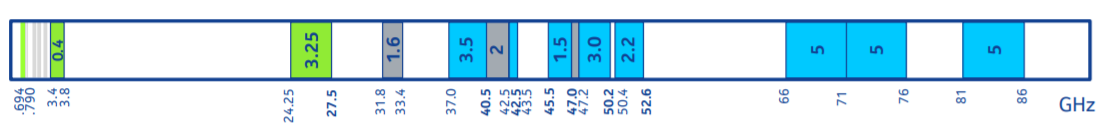
\includegraphics[width=0.95\textwidth]{./media/image5.png}
		\caption{Possible future 5G bands. Nokia\cite{1-20}}
	\end{Center}
\end{figure}


%%%%%%%%%%%%%%%%%%%% Figure/Image No: 5 Ends here %%%%%%%%%%%%%%%%%%%%

\subsection*{Sub1 GHz}
%\addcontentsline{toc}{subsubsection}{Sub1 GHz}
Lower frequencies propagate further in the environment, and therefore it is possible to cover more area per antenna. Therefore, sub-1 GHz spectrum is needed to extend high speed 5G mobile broadband coverage across suburban and rural areas and for new services like connected cars and smart sensors.\par

In fact, there is some mobile spectrum in this range that will be used in the near future. The European Commission has already decided that 700 MHz will be used to support 5G services in Europe \cite{1-21}. Similarly, the Federal Communications Commission of the United States (FCC) has indicated that the 600 MHz band could be used to drive 5G services in the United States.\par

\subsection*{1 - 6 GHz}
%\addcontentsline{toc}{subsubsection}{1 - 6 GHz}
The spectrum from 1-6 GHz offers a mixture of coverage and capacity for 5G services. That is why there is a reasonable amount of existing mobile broadband spectrum identified within this range that could potentially be allocated to 5G technologies. \par

Using spectrum within the 3.3 and 3.8 GHz range is highly interesting for initial commercial 5G services. For example, Ofcom, the UK regulator, published in April the results of the spectrum auction for the band of 2.3 and 3,4 GHz \cite{1-22}. Other mobile bands in the 1-6 GHz range that are currently used for 3G and 4G services should be gradually refarmed for 5G. In this regard, the RSPG stated in November 2016 \cite{1-23} that 3.6 GHz (3400-3800 MHz) will be the first primary band for 5G and bring the necessary capacity for new 5G services.\par

Ofcom launched in April 2016 a Call for Inputs \cite{1-24} asking for opinions on the potential of the 3.8 to 4.2 GHz band for 5G development. However, after that consultation, Ofcom decided not to consider this band as a current priority \cite{1-25} candidate for mobile services in the UK– which is the top priority level in Ofcom strategies – but kept it in the second level: \guillemotleft high priority\guillemotright  \cite{1-26}. \par

\subsection*{Above 6 GHz}
%\addcontentsline{toc}{subsubsection}{Above 6 GHz}
Part of the usage of the networks will occur within crowded cities where networks will have to be designed for capacity rather than for coverage, so the benefits of lower frequencies will be insignificant (The main benefit is that they do propagate further than higher ones) and the differences between low and high frequencies become much less significant.\par

Higher frequencies are cheaper and not so prone to have coverage obligations as the lower ones since they are not so useful for broadcasting in long distances and no MNOs would pay for them. They also have large gaps that could be allocated for mobile broadband services quite fast, giving a significant extra bandwidth to the network. These wide bandwidths will be the key for the fastest 5G services, this part of the spectrum is intended for the ultrahigh speed mobile broadband scenario. \par

The spectrum targeted above 6 GHz is expected to comprise a mixture of licensed and unlicensed mobile bands. 5G mobile bands should be agreed at WRC-19, under Agenda Item 1.13, \cite{1-27} which is considering the following bands for 5G: 24.25-27.5 GHz, 31.8-33.4 GHz, 37-43.5 GHz, 45.5-50.2 GHz, 50.4-52.6 GHz, 66-76 GHz and 81-86 GHz. However, some countries are also investigating other mobile bands above 6 GHz for 5G services, which will not be considered at WRC-19.\par

In November 2016, the Radio Spectrum Policy Group (RSPG) of the European Commission pointed out that the pioneer band in this range will be 26 GHz (24.25-27.5 GHz) \cite{1-23}, which they describe as the band that will \guillemotleft \textit{provide ultra-high capacity for innovative new services, enabling new business models and sectors of the economy to benefit from 5G}\guillemotright .\par

\subsection*{The importance of the 700 MHz band}
%\addcontentsline{toc}{subsubsection}{The importance of the 700 MHz band}
The 700 MHz band will have a key role in this paper due to a combination of two factors. As it has been introduced in previous chapters, once it is reallocated, it will be the band with the best propagation properties available for mobile communications in Europe. Now that all urban areas benefit from high-speed mobile connections, the European Union is giving top priority to the development of high-speed access in suburban and rural areas \cite{1-28}. Apart from that, the fact that the second digital dividend is a reality in most countries of Europe, it will enable a faster roll-out of the 5G of mobile communications, which is expected by 2020 \cite{1-29}. \par

\section{State of the Art}
%\addcontentsline{toc}{subsection}{State of the Art}
The aim of this Master Thesis is to analyze how the actions of the regulatory bodies will affect in different ways the rollout of 5G in Europe. Hence, this chapter explores the literature related to the measures that countries have taken to foster a nationwide high-speed mobile communications access previously, with particular emphasis on mobile coverage obligations. \par

\subsection*{The weight of the spectrum’s price factors}
%\addcontentsline{toc}{subsubsection}{The weight of the spectrum’s price factors}
Insua et. al explores in \cite{1-30} the parameters that determine the price that mobile operators pay for radio spectrum in some European countries and applies multiple regression analysis to generate a model that, based on parameter combinations, predicts the outcome of spectrum auctions when they have not taken place yet.\par

In this paper, Insua et al state that the main factors that affect the price of the spectrum are the frequency band and the country in which the auction is taking place, while other factors such as the number of competitors or the year in which this bidding takes place have a minor impact. The following table shows the adjusted R as a measurement of the relation between the variable and the price of the spectrum:


%%%%%%%%%%%%%%%%%%%% Figure/Image No: 6 starts here %%%%%%%%%%%%%%%%%%%%

\begin{figure}[H]
	\begin{Center}
		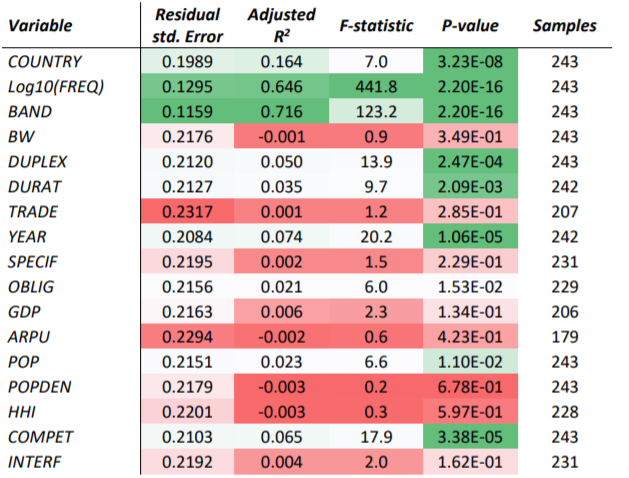
\includegraphics[width=0.95\textwidth]{./media/image6.png}
		\caption{Factors of the bids amounts in spectrum auctions. Insua et. al\cite{1-30}}
	\end{Center}
\end{figure}


%%%%%%%%%%%%%%%%%%%% Figure/Image No: 6 Ends here %%%%%%%%%%%%%%%%%%%%

\subsection*{The usage of spectrum aggregation limits}
%\addcontentsline{toc}{subsubsection}{The usage of spectrum aggregation limits}
The work by Cave $\&$  Webb \cite{1-31} for the FCC (Federal Communications Commission) of the United States analyzes the spectrum caps imposed by the European regulators. Despite the reluctance in the United States to use spectrum-aggregation limits based on the belief that it would reduce the price of the spectrum, the study states that almost all European regulators established one.\par

According to the paper, European regulators looked for a balance between raising revenues and fostering competition by setting a spectrum cap that limits the amount of spectrum for which one MNO can bid. The study reveals that there was \textit{\guillemotleft no difference between auctions where limits were hit and the case where the limit was not\guillemotright } and they also state that \guillemotleft \textit{there is no evidence that [spectrum caps] do materially reduce revenue\guillemotright .}\par

\subsection*{Ofcom: Connected Nations 2017}
%\addcontentsline{toc}{subsubsection}{Ofcom: Connected Nations 2017}
This Ofcom´s annual report, published in December 2017, analyzes the evolution of the coverage of broadband and mobile networks of the UK in 2017 \cite{1-32}. They define that an area has data services coverage when \guillemotleft \textit{Nearly all connections [95$\%$  of the time] should deliver a speed of at least 2Mbit/s. This is fast enough to allow users to browse the Internet and watch the glitch-free mobile video\guillemotright .}\par

This report states that the indoor coverage at home or at the office is of 85$\%$  for mobile data services,\ while outdoor is of just 63$\%$ .  Ofcom has also a category for coverage in roads in which they set it to 58$\%$ . This category considers the reduction of mobile signal levels as they travel through the metal frame of the vehicle and is a key measure due to the increased interest in connected cars which will be possible thanks to the 5G technologies.\par

Ofcom also compares the coverage per nation in the UK and warns about the difference in coverage between urban and rural areas and between England and other nations. Northern Ireland has a greater proportion of dispersed properties throughout the countryside, making it more difficult to deliver a proper indoor coverage. In fact, it is the only nation that has a better outdoor data services coverage than indoor. On the other side, in Scotland, with low population densities and large and often mountainous areas, geographic outdoor coverage is so low, while the indoor coverage is reasonably good. \par

Based on these results and the strategical aspect of the data mobile services, Ofcom states the necessity of setting coverage obligations to minimize the difference between nations and regions of the UK.



%%%%%%%%%%%%%%%%%%%% Figure/Image No: 7 starts here %%%%%%%%%%%%%%%%%%%%

\begin{figure}[H]
	\begin{Center}
		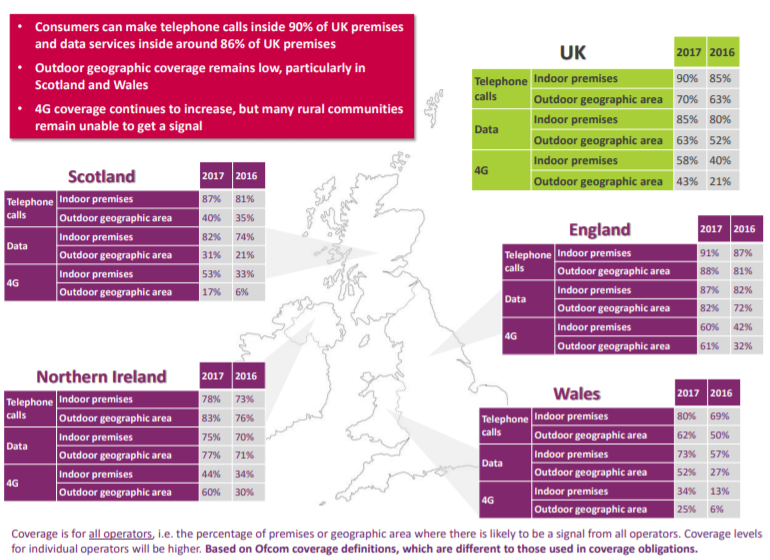
\includegraphics[width=0.95\textwidth]{./media/image7.png}
		\caption{Ofcom analysis of operator coverage, June 2017\cite{1-32}}
	\end{Center}
\end{figure}


%%%%%%%%%%%%%%%%%%%% Figure/Image No: 7 Ends here %%%%%%%%%%%%%%%%%%%%

\subsection*{Technical analysis of the cost of extending an 800 MHz mobile broadband coverage obligation for the UK}
%\addcontentsline{toc}{subsubsection}{Technical analysis of the cost of extending an 800 MHz mobile broadband coverage obligation for the UK}
This document produced by Real Wireless on behalf of Ofcom \cite{1-33} examines the investment effort that MNOs must carry out in the UK to comply with the coverage obligations imposed by Ofcom to the operator that won the spectrum block with coverage obligations in the 800 MHz auction in 2013. This analysis provides some important insights for this Master Thesis:\par

\begin{itemize}
	\item According to this analysis, upgrading existing sites in the UK to use a block of 5 MHz 800 MHz would be as low as 61$\%$  of indoor coverage obligation.\par

	\item Rising the transmit power will not imply a significant coverage gain since gains are limited due to terrain and uplink limitations.\par

	\item Costs of achieving a specific indoor coverage are approximately 20$\%$  lower using 2 blocks of 10 MHz that using 2 blocks of 5 MHz in the 800 MHz band.\par

	\item The marginal cost of rising the indoor coverage from 95$\%$  to 98$\%$  is greater than the required to increase the coverage from 90$\%$  to 95$\%$ .
\end{itemize}\par

